\chapter{Dise\~no}
%

%%%%%%%%%%%%%%%%%%
\section{Software}
%%%%%%%%%%%%%%%%%%
\subsection{Dise\~no de alto nivel}
%%%%%%%%%%%%%%%%%%%%%%%%%%%%%%%%%%%
%
Lo primero a considerar es la forma de comunicaci\'on entre la computadora y
la impresora, y si bien el dise\~no debe centrarse en mantener los costos de
producci\'on y construcci\'on bajos de nada sirve un dispositivo basado en
tecnolog\'ia a en desuso o pronta a desaparecer. Es por esto que en vez de
elegir m\'etodos convencionales como lo pueden ser el protocolo serial
R232\footnote{V\'ease - \url{http://es.wikipedia.org/wiki/RS-232}} o
paralelo\footnote{V\'ease - \url{http://es.wikipedia.org/wiki/Puerto_paralelo}}
(t\'ipico de impresoras antiguas), se usar\'a el protocolo serie de
comunicaci\'on \emph{USB}\footnote{El est\'andar se explica en detalle en
\fullref{cap:usb}.} \'Este est\'andar se encuentra en la mayor\'ia de los
equipos actuales y provee una versatilidad y flexibilidad como pocos.\\

Otro tema muy importante a considerar es el sistema operativo a usar en la
computadora. Si bien puede pensarse como respuesta obvia el sistema operativo
de Microsoft,
Windows\footnote{V\'ease - \url{http://www.microsoft.com/spain/windows/}} (en
su versi\'on m\'as comercializada \emph{XP}), este enfoque fuerza al potencial
usuario a comprar una licencia\footnote{Dichas licencias rondan los 100 US\$}
solo para poder utilizar la impresora.\
Entonces en vez de optar por un sistema pago se usar\'a el sistema
operativo \emph{GNU/Linux}
% ###--->>> Poner referencia a la secci\'on donde hablo de gnu/linux
del cual existen mas de mil versiones distintas, la mayor\'a de ellas
gratuitas.
De esta forma el usuario puede obtener una copia de este sistema operativo
gratuito y usar la impresora sin mayores restricciones.\\

En la figura \ref{fig:pc_usb_printer} se muestra un esquema b\'asico de lo
dicho
anteriormente. El esquema en su m\'as alto nivel ser\'a usar una computadora
con \emph{GNU/Linux} como sistema operativo y una conexi\'on mediante
\emph{USB} al dispositivo.

\begin{figure}[htp]
\centering
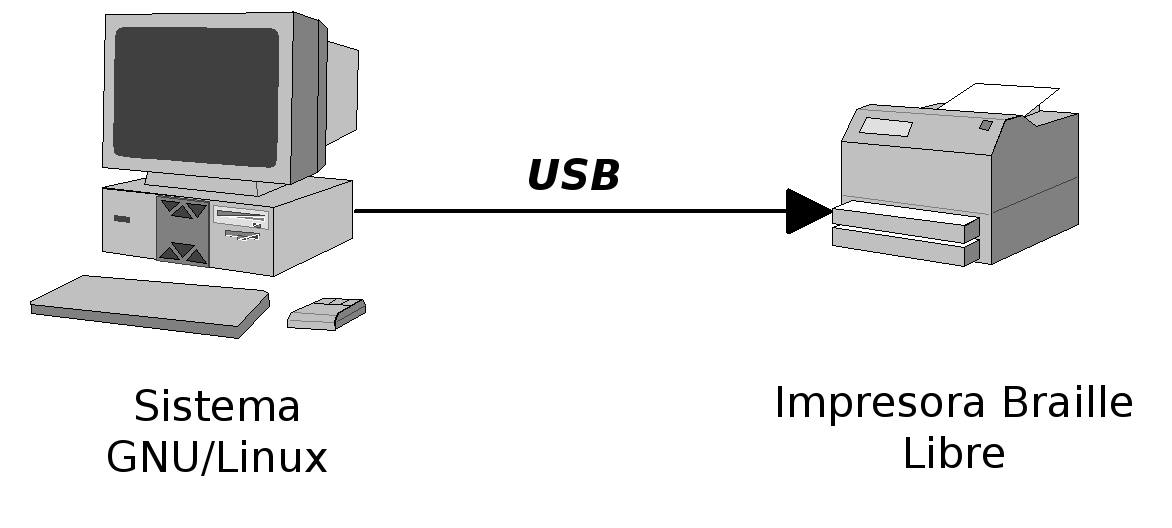
\includegraphics[width=13cm]{./img/pc_usb_printer.png}
\caption{S.O, conexi\'on e impresora}
\label{fig:pc_usb_printer}
\end{figure}

%%%%%%%%%%%%%%%%%%%%%%%%%%%%%%%%%
\subsection{Dise\~no de nivel medio}
%%%%%%%%%%%%%%%%%%%%%%%%%%%%%%%%%
%


%%%%%%%%%%%%%%%%%%%%%%%%%%%%%%%
\subsubsection{Entradas y salidas}
%
Si bien no se encuentra dentro del alcance de este trabajo proveer una
soluci\'on para la parte mec\'anica de la impresora, es necesario determinar
con que debe interactuar la parte electr\'onica, esto es; cuales ser\'an las
entradas y cuales ser\'an las salidas.\\

Como se determin\'o anteriormente el mecanismo a usar ser\'a de un \'unico
punz\'on desplazante, esto implica que se debe generar moviemiento horizontal
para el cabezal y movimiento vertical para el papel, es necesaria adem\'as una
se\~nal para manejar el punz\'on. Quedan entonces definidas las salidas.\
Por otra parte es necesario definir algun tipo de se\~nal de entrada. Para
mantener un dise\~no simple solo se usar\'an entonces una se\~nal de presencia
de papel y un fin de carrera para el cabezal.\\

En la figura \ref{fig:pc_uc_motors} se ve el dise\~no general. \'Este posee la
particularidad de ser el usado por la mayoria de las antiguas impresoras
matriz de punto, siendo entonces posible usar un mecanismo fabricado a medida,
o bien adaptar una impresora vieja.


\begin{figure}[htp]
\centering
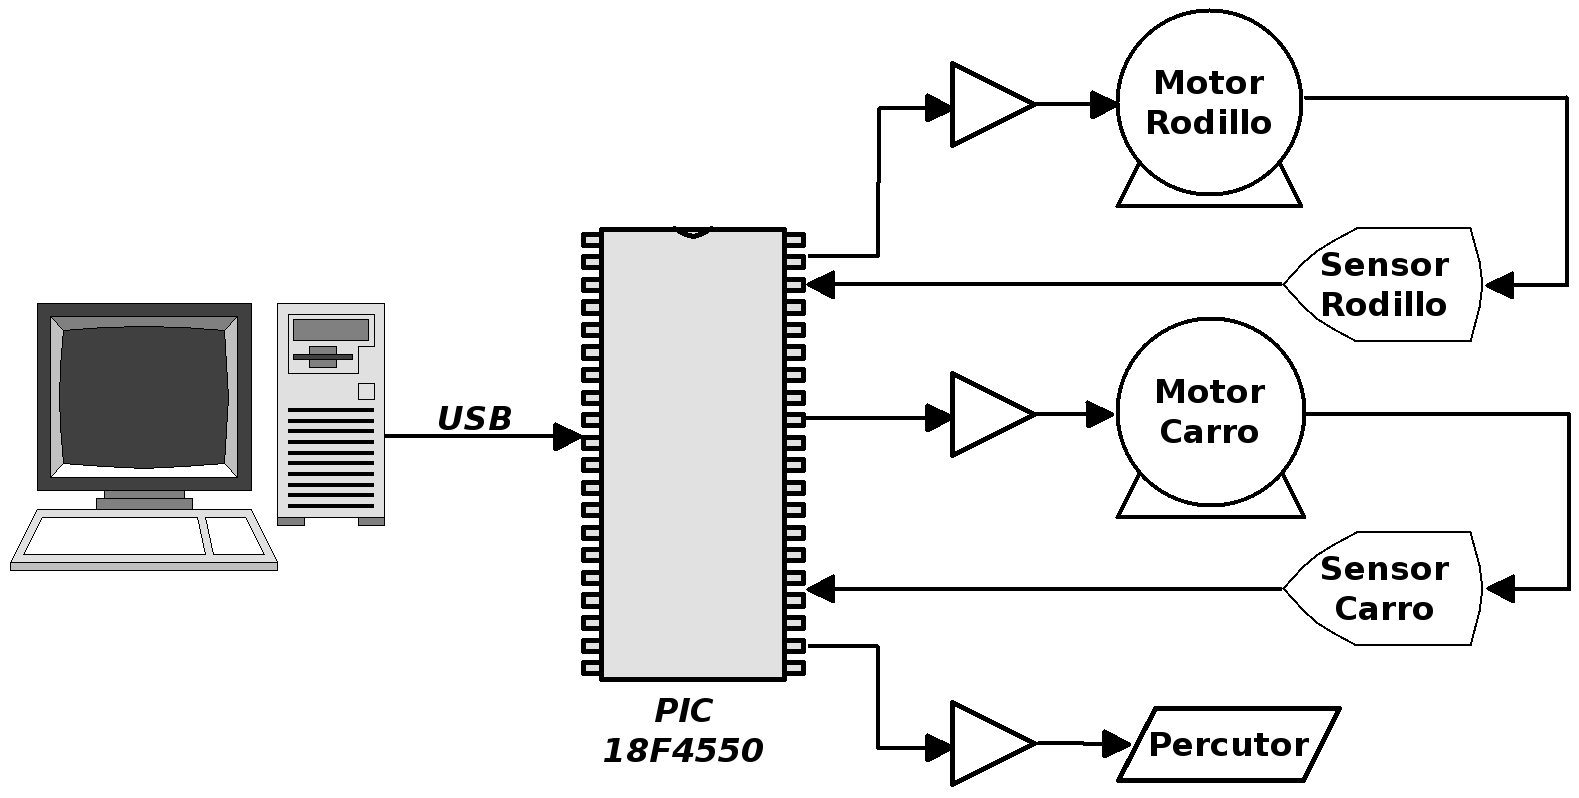
\includegraphics[width=13cm]{./img/pc_uc_motors.png}
\caption{Dise\~no de alto nivel.}
\label{fig:pc_uc_motors}
\end{figure}



%%%%%%%%%%%%%%%%%%%%%%%%%%%%%%%%%%%
\subsection{Dise\~no de bajo nivel}
%%%%%%%%%%%%%%%%%%%%%%%%%%%%%%%%%%%
%
Para mantener los costos bajos, y teniendo en cuenta las limitaciones del
microcontrolador elegido, la mayor parte del procesamiento se lleva a cabo
en la computadora, logrando de esta manera economizar espacio en el firmware y
evitar la neceidad de hardware extra.\\

En su mayoria, las impresoras braille comerciales posen integrado un sistema
sintetizador de voz, con mensajes pregrabados en varios idiomas que se
reproducen por cada acci\'on que la impresora ejecuta. Esto, claro est\'a,
implica la necesidad de grandes cantidades de memoria y quiz\'a un chip
dedicado. Para evitar usar chips sintetizadores de voz y memeorias, y
teniendo en cuenta que la mayoria de las computadoras actuales poseen sistemas
de reproducc\'on de audio, \'este trabajo queda a cargo de \'estas.\
Al igual que el audio, existe gran cantidad de prcesamiento a llevar a cabo
para la conversi\'on del texto a braille, y varias decisiones que usualmente
toman las impresoras. Todo esto se resuelve del lado de la computadora.\
Entonces es posible ahora, hablar de driver (que ser\'a el programa
ejecutandose en la computadora) y firmware (que ser\'a el programa ejecutandose
en el microcontrolador) al referirnos a la computadora y a el dispositivo
respectivamente.\
Para lograr esto, el firmware solo es capaz de realizar tareas basicas y
sencillas, respondiendo a instrucciones que el driver envia y reportando los
resultados obtenidos. La figura \ref{fig:driver_firmware} muestra una
representaci\'on de lo dicho anteriormente.\\

\begin{figure}[htp]
\centering
\begin{tikzpicture}[node distance = 10cm, auto]
  \node [block] (driver) {Driver};
  \node [block, right of=driver] (firmware) {Firmware};
  \draw [line] (driver) to [bend right] node [midway] {Datos} (firmware);
  \draw [line] (driver) to [bend left] (firmware) node [midway]
{Instrucciones};
  \draw [line] (firmware) -- node [midway] {Resultados} (driver);
\end{tikzpicture}
\caption{Canales de comunicaci\'on entre el driver y el firmware.}
\label{fig:driver_firmware}
\end{figure}


Para instanciar el modelo anterior haciendo uso del m\'etodo de comunicaci\'on
elegido\footnote{Esto es el estandar USB}, se definen dos
endopoints\footnote{V\'ease \fullref{cap:usb_endpoints}} bidireccionales, uno
dedicado exclusivamente al envio de datos (endpoint 1 o EP1) y otro para enviar
instucciones y recibir resultados (endpoint 2 o EP2). La figura
\ref{fig:driver_eps_firmware} muestra la comunicaci\'on mediante endpoints.


\begin{figure}[htp]
\centering
\begin{tikzpicture}[node distance = 10cm, auto]
  \node [block] (driver) {Driver};
  \node [block, right of=driver] (firmware) {Firmware};
  \draw [line] (driver) (1.2,0.6) -- (8.8,0.6) node [midway] {Datos - EP1}
(firmware);
  \draw [line] (driver) (1.2,0) -- (8.8,0) node [midway] {Instrucciones - EP2
Out} (firmware);
  \draw [latex-] (firmware) (1.2,-0.6) -- (8.8,-0.6) node [midway]
{Resultados - EP2 In} (driver);
\end{tikzpicture}
\caption{Canales de comunicaci\'on entre el driver y el firmware mediante
endpoints.}
\label{fig:driver_eps_firmware}
\end{figure}

Habiendo definido los canales de comunicaci\'on y sus respectiva funciones, es
necesario determina el tipo y forma de los datos y las instrucciones a manejar.

\subsubsection{Datos}
%%%%%%%%%%%%%%%%%%
%
La cantidad de caracteres braille que entran en el ancho de una hoja A4, ronda
los 30 dependiendo del tama\~no de las sangrias. Para dejar un margen se eligen
28 caracteres. Teniendo en cuenta que los caracteres braille poseen dos
columnas de puntos\footnote{V\'ease \fullref{cap:braille_cell}} y que el
dato m\'inimo que se puede enviar por USB es de un byte\footnote{V\'ease
\fullref{cap:usb_byte}}, para completar una linea a lo ancho de una p\'agina de
una fila de puntos se necesitan:

\begin{center}
$28 caracteres * 2 puntos = 56 bits$\\
$56 bits / 8  = 7 bytes$
\end{center}

\begin{table}[ht]
\centering
\begin{tabular}{|c|c|c|} \hline
\braille{c} \braille{c} \braille{c} \braille{c} &
\braille{c} \braille{c} \braille{c} \braille{c} &
... 												 \\ \hline
byte 1 & byte 2 & ...\\ \hline
\end{tabular}
\caption{Bytes por puntos braille} 
\label{tab:bytes_braille}
\end{table}

Entonces el m\'aximo numero de bytes a enviar por linea es de 7 bytes.\
Para formar una fila completa de caracteres, es necesario realizar tres
envios, ya que los caracteres braille poseen tres filas de
puntos\footnote{V\'ease \fullref{cap:braille_cell}}, lo cual genera 21 bytes
($7bytes*3$) por fila, y un total de 588 ($21bytes * 28filas$) bytes por
p\'agina ya que en una hoja A4 se suelen imprimir 28 filas de caracteres. 

\subsubsection{Instrucciones}
%%%%%%%%%%%%%%%%%%%%%%%%%%
%
Para limitar la capacidad de funcionalidades del dispositivo solo se
definen ocho instrucciones b\'asicas descriptas en la tabla
\ref{tab:instructions_set}.

\begin{table}[ht]
\centering
\begin{tabular}{|l|c|l|} 												\hline
\rowcolor[gray]{.9}
Instrucci\'on & Byte & Descripci\'on 								\\ 	\hline
RESET 		&	0x01	&	Resetea el cabezal	al punto de origen	\\	\hline
PRINT 		&	0x02	&	Imprime los datos						\\	\hline
MOV\_SHORT 	&  	0x03	&	Desplaza el cabezal entre puntos		\\	\hline
MOV\_LONG  	&  	0x04	&	Desplaza el cabezal entre caracteres	\\	\hline
ROT\_SHORT 	&	0x05	&	Rota el rodillo entre lineas			\\	\hline
ROT\_LONG   &	0x06	&	Rota el rodillo entre caracteres		\\	\hline
PULL\_PAPER	&	0x07	&	Rota el rodillo hasta sacar el papel	\\	\hline
STATUS		&	0x08	&	Pide el estado de los sensores			\\	\hline
\end{tabular}
\caption{Instrucciones de impresi\'on} 
\label{tab:instructions_set}
\end{table}

Este set de instrucciones proporcionan todas las funcionalidades necesarias
para poder llevar a acabo un proceso de impresi\'on normal.

\subsubsection{Resultados}
%%%%%%%%%%%%%%%%%%%%%%%
%
Se definen dos tipos de resultados distintos, uno que es devuelto cuando se
envia la instruccion \emph{STATUS} y otro que se genera siempre luego de un
envio de datos que consta en el dato recreado por la impresora, esto es solo a
modo de verificaci\'on tipo \emph{echo}.\\

Ante una instrucci\'on del tipo \emph{STATUS}, el dispositivo lee los estados
de los dos sensores y genera un byte de reporte descripto en la tabla
\ref{tab:report_byte}.


\begin{table}[ht]
\centering
\begin{tabular}{|c|c|c|c|c|c|c|c|}									\hline
\multicolumn{8}{|c|}{Byte}										\\	\hline
x & x & x & x & x & x & 1/0 & 1/0 								\\ 	\hline
- & - & - & - & - & - & Sensor de cabezal & Sensor de papel		\\	\hline
\end{tabular}
\caption{Byte de reporte} 
\label{tab:report_byte}
\end{table}

Entonces dependiendo del estado de los dos bits menos significativos del byte
de reporte, el driver puede saber en que estado se encuentra la impresora.\\

El segundo tipo de resultado definido es el \emph{echo}. Cuando el driver
envia datos para imprimir, la impresora comienza el proceso de impresi\'on y
recrea los datos recibidos segun lo que hace, luego este dato recreado
se envia de vuelta al driver quien comprar ambos datos y verifica que sean
iguales, la figura \ref{fig:rec_dat} muestra un diagrama simplificado de este
proceso.

\begin{figure}[htp]
\centering
\begin{scriptsize}
\begin{tikzpicture}
  [auto,
   decision/.style={diamond, draw=blue, thick, fill=blue!20,
                    text width=9em, text badly centered,
                    inner sep=1pt},
   block/.style   ={rectangle, draw=blue, thick, fill=blue!20,
                    text width=10em, text centered, rounded corners,
                    minimum height=4em},
   line/.style    ={draw, thick, -latex' ,shorten >=2pt},
   cloud/.style   ={draw=red, thick, ellipse,fill=red!20,
                    minimum height=2em}]
  \matrix [column sep=10mm,row sep=7mm]
  {
    % row 1
      \node [cloud] (driver)   		{Driver}; & 
		&
      \node [cloud] (firmware) 		{Firmware}; \\
    % row 2
	  \node [block] (dat_send_d)	{Envio del dato a imprimir \(\$dat_d\)}; &
		&
      \node [block] (dat_resv_f)	{Recepci\'on del dato \(\$dat_d\)}; \\
    % row 3
     	& &
      \node [block] (print) 		{Proceso de impresi\'on y
reconstrucci\'on del dato \(\$dat_d -> \$dat_f\)};  \\
    % row 4
	\node	[block]	(dat_resv_d)	{Recepci\'on del dato reconstruido
	\(\$dat_f\)};
		& &
	  \node [block] (dat_send_f)	{Envio del dato reconstruido \(\$dat_f\)};
\\
  };
  \begin{scope}[every path/.style={draw, -latex'}]
    \path	(dat_send_d) -- (dat_resv_f) node [midway] {EP1 Out};
    \path	(dat_resv_f) -- (print);
    \path   (print)      -- (dat_send_f);
    \path   (dat_send_f) -- (dat_resv_d) node [midway] {EP2 In};;
  \end{scope}
\end{tikzpicture}
\end{scriptsize}
\caption{Proceso de recontrucci\'on de datos}
\label{fig:rec_dat}
\end{figure}

%%%%%%%%%%%%%%%%%%%%%%%%%%%%%%%%%%%%%%%%%%%%%%%%%%%%%%%%%%%%%%%%%%%%%%%%%%%%%%%
%%%%%%%%%%%%%%%%%%%%
\section{Hardware} %
%%%%%%%%%%%%%%%%%%%%
%
\subsection{Dise\~no de alto nivel}
%%%%%%%%%%%%%%%%%%%%%%%%%%%%%%%%%%%
%
Para mantener la simplicidad del dise\~no se utiliza un metodo modular, de tal
manera de independizar las soluciones y focalizar los problemas.\
Es facilmente divisible el dise\~no en dos grandes areas; control y potencia.\\

La parte de control se encarga principalmente en establecer la conexi\'on con
la computadora, procesar los datos y generar las se\~nales de control.\
La parte de potencia es la encargada de manejar los motores, sensores y el
punz\'on.\\

El mantener ambos dise\~nos independientes provee la flexibilidad necesaria
para mantener bajos costos y sencillez de implementaci\'on.





%%%%%%%%%%%%%%%%%%%%%%%%%%%%%
\subsubsection{Microcontrolador}
Lo primero a analizar es el microcontrolador a usar. El mercado de
desarrollo electr\'onico Argentino tiene una tendencia a usar las soluciones de
Microchip\footnote{V\'ease - \url{http://www.microchip.com/}}, y es por ello
que existe mucha gente capacitada en los microcontroladores de esta empresa, y
si bien sus productos no son los mejores del mercado internacional, sus
precios son bastantes competitivos al igual que las funcionalidades que
prestan y la amplia gama de variedades que poseen.\

Como el objetivo de este trabajo se enfoca en el mercado local y el bajo costo
de producci\'on, los productos de Microchip se presentan como la mejor
alternativa.\\

El requerimiento primario para elegir el microcontrolador a usar es que posea
soporte USB. La familia \emph{18FXXXX}\footnote{V\'ease - \url{
http://www.microchip.com/stellent/idcplg?IdcService=SS_GET_PAGE&nodeId=2654}}
satisface este requerimiento. De esta familia los dos microcontroladores m\'as
comercializados\footnote{Esto implica facilidad a la hora de conseguir en el
mercado local.} en el pa\'is son el \emph{18F2550} y el \emph{18F4550}. La
tabla \ref{tab:table_12_14} muestra las principales caracter\'isticas de ambos
microcontroladores.

\begin{table}[htp]
\begin{scriptsize}
\centering
% use packages: array,booktabs
\begin{tabular*}{\textwidth}{@{\extracolsep{\fill}}|l|c|c|} \hline
 \rowcolor[gray]{.9}
 & 18F2550 & 18F4550 												\\ \hline 
 Program Memory Type & Flash & Flash								\\ \hline
 Program Memory (KB) & 32 & 32										\\ \hline
 CPU Speed (MIPS) & 12 & 12											\\ \hline
 RAM Bytes & 2048 & 2048											\\ \hline
 Data EEPROM (bytes) & 256 & 256									\\ \hline
 Digital Communication Peripherals & 1-A/E/USART, 1-MSSP(SPI/I2C) &
1-A/E/USART, 1-MSSP(SPI/I2C) 										\\ \hline
 Capture/Compare/PWM Peripherals & 2 CCP &  CCP, 1 ECCP 			\\ \hline
 Timers & 1 x 8-bit, 3 x 16-bit & 1 x 8-bit, 3 x 16-bit 			\\ \hline
 ADC & 10 ch, 10-bit & 13 ch, 10-bit								\\ \hline
 Comparators & 2 & 2 												\\ \hline
 USB (ch, speed, compliance) & 1, Full Speed, USB 2.0 & 1, Full Speed, USB 2.0
																	\\ \hline
 Temperature Range (C) & -40 to 85 & -40 to 85  					\\ \hline
 Operating Voltage Range (V) & 2 to 5.5 & 2 to 5.5					\\ \hline
 Pin Count & 28 & 40												\\ \hline
\end{tabular*}
\caption{Comparaci\'on PIC18F2550 y PIC18F4550} 
\label{tab:table_12_14}
\end{scriptsize}
\end{table}


Se observa que no existe gran diferencia entre ambos MCU\footnote{Del ingles
\emph{Micro Controller Unit}}, al igual que sus precios como se observa en la
tabla \ref{tab:table_12_14_price}.

\begin{table}[htp]
\centering
\begin{tabular}{l|r}
 \toprule
  MCU & US\$		\\ \hline
 18F2550 & 2.39  	\\ 
 18F4550 & 3.65 	\\
 \bottomrule
\end{tabular}

\begin{tiny} 
\caption{Comparaci\'on de precios PIC18F2550 y PIC18F4550}\footnote{Los precios
unitarios fueron extraidos de la p\'agina oficial de Microchip}
\end{tiny} 
\label{tab:table_12_14_price}
\end{table}

Se puede concluir entonces que para \'este trabajo el PIC18F2550 satisface en
grandes rasgos los requerimientos m\'inimos. No obstante, y por cuestiones de
comodidad\footnote{Esto es disponibilidad a la hora de realizar el proyecto.}
,se usar\'a el PIC18F4550, realizando el dise\~no con vistas a migrar el MCU
al PIC18F2550 en el futuro.\\



\subsection{Potencia}
%%%%%%%%%%%%%%%%%%%%%
%
El modulo de potencia se focaliza principalmente en el manejo de los motores y
sensores de la impresora.

\subsubsection{Motores}
%%%%%%%%%%%%%%%%%%%%%%%
%
Como muestra la figura \ref{fig:pc_uc_motors}, solo se controlan dos motores, y
para mejor precis\'on y mantener el dise\~no compatible con impresoras viejas
matriz de punto, los motores \emph{paso a paso} son la mejor elecci\'on.\\

Existen dos grandes tipos de motores paso a paso; \emph{bipolares} y
\emph{unipolares}. La figura \ref{fig:stepper_motors} muestra la disposici\'on
y conexi\'on de los devanados de ambos tipos de motores. 


%http://www.electojects.com/motors/02440.gif
\begin{figure}[htp]
\centering
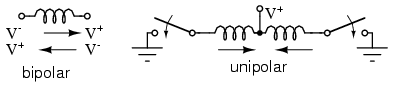
\includegraphics[scale=0.7]{./img/02440.png}
\caption{Motores paso a paso.}
\label{fig:stepper_motors}
\end{figure}

Claramente la desventaja que presentan los motores \emph{bipolares} frente a
los \emph{unipolares} es que necesitan invertir el sentido de la corriente en
sus bobinados, esto implica mayor complejidad en el circuito controlador.\
Y en contra partida la mayor ventaja de los motores \emph{unipolares} radica
(mas alla de la simpleza del circuito controlador) en que eran los mas
usados\footnote{Y son mas faciles de encontrar en el mercado local} en la
antiguas impresoras matriz de punto, lo cual es un beneficio mas que importante
para este trabajo.\
Para satisfacer los dos movimientos mec\'anicos necesarios (rotaci\'on del
rodillo de papel y desplazamiento horizontal del cabezal) el dise\~no requiere
controlar dos motores paso a paso unipolares individuales.\
Entre los motores paso a paso \emph{unipolares}, los mas usados son los de
cuatro fases, mas comunmente denominados \emph{motor de cinco cables}. La
figura \ref{fig:stepper_motor_5_wire} muestra simb\'olicamente la distribucion
interna de los devanados de este tipo de motores.

% http://www.piclist.com/images/member/RB-ezy-Q33/5wire.GIF
\begin{figure}[htp]
\centering
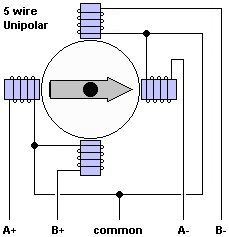
\includegraphics[scale=0.5]{./img/5wire.png}
\caption{Motor unipolar paso a paso de 4 fases.}
\label{fig:stepper_motor_5_wire}
\end{figure}

Para lograr la rotaci\'on, cada bobina debe ser energizada de forma
independiente y siguiendo una secuancia particular. El circuito de la figura
\ref{fig:cir_single_coil} satisface los requisitos minimos para energizar una
\'unica bobina.

\begin{figure}[htp]
\centering
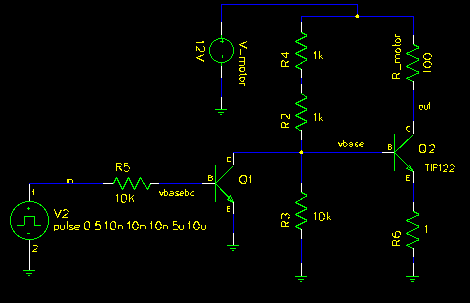
\includegraphics[scale=0.7]{./img/cir_single_coil.png}
\caption{Circuito de potencia para una bobina de motor paso a paso unipolar.}
\label{fig:cir_single_coil}
\end{figure}

El divisor resistivo \emph{R2 R3} es una resistencia variable, que junto con
la resistencia de emisor de 1 \ohm  permiten controlar la corriente que circula
por la bobina, de esta manera este circuito puede ser ser usado por diversos
motores de diversas impedancias. Debido a que el el circuito de salida se
conecta directamente a la bobina del motor, y esta puede ser de muy baja
impedancia, el transistor de salida debe ser capaz de manejar corrientes altas,
en este caso se hace uso de un \emph{TIP122}.\
La figura \ref{fig:cir_single_coil_plot} muestra las diferentes tensiones que
actuan en el circuito. 

\begin{figure}[htp]
\centering
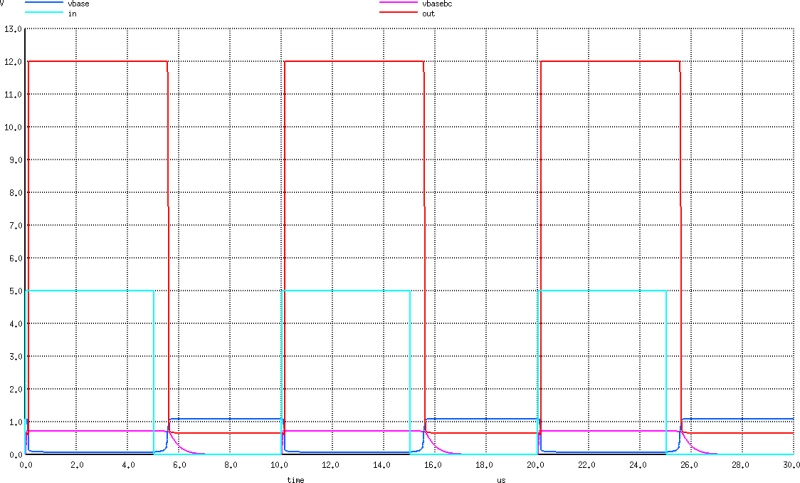
\includegraphics[width=15cm]{./img/cir_single_coil_plot.png}
\caption{Simulaci\'on del circuito de potencia para una bobina de motor paso a
paso unipolar.}
\label{fig:cir_single_coil_plot}
\end{figure}

Un motor paso a paso unipolar de cuatro fases tiene cuatro bobinas, para
manejar los dos motores es necesario luego replicar ocho veces este circuito.
El esquematico final se encuentra en el anexo en \fullref{cap:driver_schema}.






\subsubsection{Sensores}
%%%%%%%%%%%%%%%%%%%%%%%
%
El requerimiento de los sensores es bastante sencillo; como fue definido
anteriormente, solo son necesarios dos sensores de tipo \emph{on/off}. \
Existe en el mercado un vasta variedad de interruptores que cumplen con las
condiciones necesarias y a su vez cubren un gran rango de precios.\\











%##### WTF!!!!???? #########
%\pgfmathsetseed{1}
%\foreach \col in {black,red,green,blue}
%{
%  \begin{tikzpicture}[x=10pt,y=10pt,ultra thick,baseline,line cap=round]
%    \coordinate (current point) at (0,0);
%    \coordinate (old velocity) at (0,0);
%    \coordinate (new velocity) at (rand,rand);
%    \foreach \i in {0,1,...,100}
%    {
%      \draw[\col!\i] (current point)
%     .. controls ++([scale=-1]old velocity) and
%                   ++(new velocity) .. ++(rand,rand)
%         coordinate (current point);
%      \coordinate (old velocity) at (new velocity);
%      \coordinate (new velocity) at (rand,rand);
%    }
%  \end{tikzpicture}
%}
%\begin{tikzpicture}[x=3.8cm/360]
%  \pgfplothandlerlineto
%  \pgfplotfunction{\x}{0,5,...,360}{\pgfpointxy{\x}{sin(\x)+sin(3*\x)}}
%  \pgfusepath{stroke}
%\end{tikzpicture}





